\documentclass[11pt,a4paper]{article}
\usepackage[utf8]{inputenc}
\usepackage{geometry}
\geometry{margin=1in}
\usepackage{hyperref}
\usepackage{xcolor}
\usepackage{enumitem}
\usepackage{titlesec}
\usepackage{amssymb}
\usepackage{tikz}
\usepackage{graphicx}
\usetikzlibrary{shapes.geometric, arrows, positioning}

% Colors
\definecolor{primary}{RGB}{37, 99, 235}
\definecolor{secondary}{RGB}{71, 85, 105}
\definecolor{boxbg}{RGB}{241, 245, 249}
\definecolor{boxborder}{RGB}{148, 163, 184}

% Hyperlink setup
\hypersetup{
    colorlinks=true,
    linkcolor=primary,
    filecolor=primary,      
    urlcolor=primary,
}

% Title format
\titleformat{\section}{\Large\bfseries\color{primary}}{}{0em}{}[\titlerule]
\titleformat{\subsection}{\large\bfseries\color{secondary}}{}{0em}{}

% TikZ Styles
\tikzstyle{process} = [rectangle, rounded corners, minimum width=3cm, minimum height=1cm, text centered, align=center, draw=boxborder, fill=boxbg, font=\small\bfseries]
\tikzstyle{arrow} = [thick,->,>=stealth, color=secondary]
\tikzstyle{db} = [cylinder, shape border rotate=90, aspect=0.25, draw=boxborder, fill=boxbg, minimum height=1.5cm, minimum width=2cm, text centered, font=\small\bfseries]

\begin{document}

\begin{center}
    {\Huge \bfseries StellarFlow} \\[0.5cm]
    {\Large Enterprise Treasury Operating System} \\[0.5cm]
    \textbf{Developer:} Bibek Das \\
\end{center}

\vspace{0.3cm}

\section*{Project Overview}
StellarFlow is a production-grade Web3 dashboard designed to solve the Just-In-Time (JIT) Liquidity problem for corporate treasuries. It aggregates funds proportionally from multiple isolated wallets and routes them through a single atomic transaction on the Stellar network.

\begin{center}
    \includegraphics[width=\textwidth]{dashboard.png}
\end{center}

\vspace{0.3cm}

\section*{Key Project Links}
\begin{itemize}[leftmargin=*, label=\textbullet]
    \item \textbf{GitHub Repository:} \url{https://github.com/Be-bibek/StellarFlow}
    \item \textbf{Live Demo:} \url{https://web3-private-production.up.railway.app/}
    \item \textbf{Smart Contract (Testnet):} \href{https://stellar.expert/explorer/testnet/contract/CC7RCRZ3JF3W2YNTQKYTRMVGVIZGLPIX6B2R7Q6HUOWDRK3IQKRQWLKT}{\texttt{CC7RCRZ3JF3W2YNTQKYTRMVGVIZGLPIX6B2R7Q6HUOWDRK3IQKRQWLKT}}
\end{itemize}

\vspace{0.5cm}

\section*{Tech Stack}
\begin{itemize}[leftmargin=*, label=\textbullet]
    \item \textbf{Frontend:} Next.js (React), Tailwind CSS, TypeScript
    \item \textbf{Backend:} Rust (Actix-Web), PostgreSQL, WebSockets
    \item \textbf{Blockchain:} Stellar (Soroban Smart Contracts), Stellar SDK
\end{itemize}

\vspace{0.5cm}

\section*{System Architecture}

\begin{center}
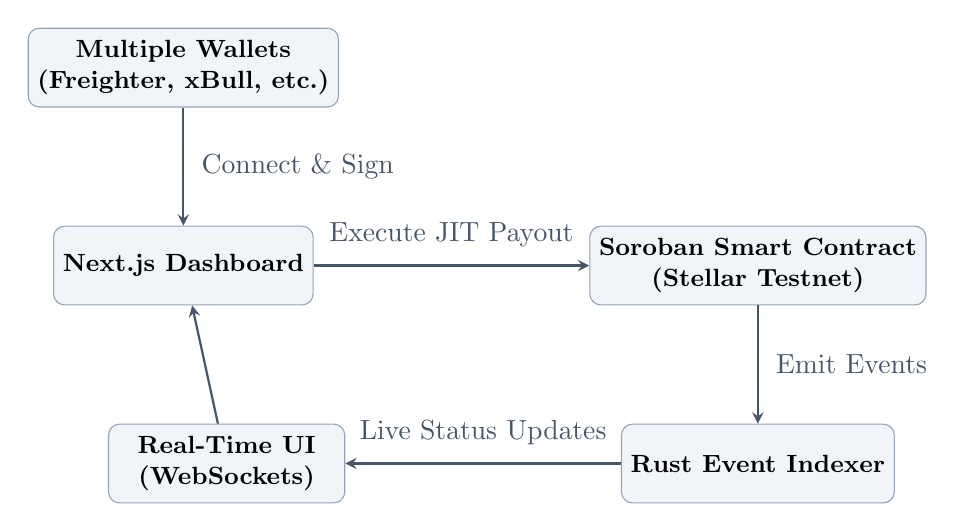
\begin{tikzpicture}[node distance=2.5cm and 4cm]
    % Nodes
    \node (wallets) [process] {Multiple Wallets \\ (Freighter, xBull, etc.)};
    \node (frontend) [process, below=1.5cm of wallets] {Next.js Dashboard};
    \node (contract) [process, right=3.5cm of frontend] {Soroban Smart Contract \\ (Stellar Testnet)};
    \node (backend) [process, below=1.5cm of contract] {Rust Event Indexer};
    \node (ui) [process, left=3.5cm of backend] {Real-Time UI \\ (WebSockets)};

    % Arrows
    \draw [arrow] (wallets) -- node[right=0.1cm] {Connect \& Sign} (frontend);
    \draw [arrow] (frontend) -- node[above=0.1cm] {Execute JIT Payout} (contract);
    \draw [arrow] (contract) -- node[right=0.1cm] {Emit Events} (backend);
    \draw [arrow] (backend) -- node[above=0.1cm] {Live Status Updates} (ui);
    \draw [arrow] (ui) -- (frontend);
\end{tikzpicture}
\end{center}

\vspace{0.5cm}

\section*{Core Deliverables Completed}

\begin{itemize}[leftmargin=0.5cm, label=$\boxtimes$]
    \item \textbf{Multi-Wallet Architecture Integration}
    \begin{itemize}[label=$\circ$]
        \item The application natively supports connecting with multiple wallet providers (Freighter, xBull, and others), breaking vendor lock-in and allowing diverse corporate actors to interact securely.
    \end{itemize}
    \vspace{0.2cm}
    
    \item \textbf{Advanced Smart Contract Deployment}
    \begin{itemize}[label=$\circ$]
        \item A highly optimized Soroban smart contract is deployed on the Stellar Testnet. It acts as an on-chain router, instantly aggregating balances across multiple treasury vaults for large payouts.
    \end{itemize}
    \vspace{0.2cm}
    
    \item \textbf{Balance \& Real-Time Transaction Tracking}
    \begin{itemize}[label=$\circ$]
        \item A comprehensive transaction history and balance verification dashboard allows users to monitor live account states. The UI reflects on-chain changes instantly via a Rust-powered WebSocket event stream.
    \end{itemize}
    \vspace{0.2cm}
    
    \item \textbf{Automated CI/CD Pipeline}
    \begin{itemize}[label=$\circ$]
        \item The project utilizes an automated Continuous Integration/Continuous Deployment (CI/CD) pipeline. This ensures that all code and smart contract logic is rigorously tested before hitting production.
    \end{itemize}
    \vspace{0.2cm}
    
    \item \textbf{Production-Ready Documentation \& Presentation}
    \begin{itemize}[label=$\circ$]
        \item The repository includes deep architectural planning documents, setup instructions, and code comments designed for enterprise handoff and rapid developer onboarding.
    \end{itemize}
    \vspace{0.2cm}

    \item \textbf{Robust Error Handling}
    \begin{itemize}[label=$\circ$]
        \item The frontend cleanly intercepts all edge cases (Wallet Rejections, Simulation Failures, Contract Reverts) and surfaces them as user-friendly notifications.
    \end{itemize}
\end{itemize}

\end{document}
